\section{Introduction}

\emph{Rule lists}, also called decision lists, are one-sided decision trees.

\section{Related work}

\citep{rivest:1987}

\citep{LethamRuMcMa15}

\citep{YangRuSe16}

\citep{garofalakis:2000-kdd,garofalakis:2000-sigkdd,garofalakis:2003}

\section{A branch-and-bound framework for optimizing rule lists}

\subsection{Rule lists for binary classification}
\label{sec:setup}

We restrict our setting to binary classification,
where rule lists are Boolean functions;
this framework is straightforward to generalize to multi-class classification.
%
Let~${\{(x_n, y_n)\}_{n=1}^N}$ denote training data,
where ${x_n \in \{0, 1\}^J}$ are binary features and ${y_n \in \{0, 1\}}$ are labels.
%
Let~${\x = \{x_n\}_{n=1}^N}$ and~${\y = \{y_n\}_{n=1}^N}$,
and let~${x_{n,j}}$ denote the $j$-th feature of~$x_n$.

A rule list ${\RL = (r_1, r_2, \dots, r_K, r_0)}$ of length~${K \ge 0}$ is a
${(K+1)}$-tuple consisting of~$K$ association rules followed by a default rule~$r_0$;
we sometimes call this a $K$-rule list.
%
An association rule~${p \rightarrow q}$ is an implication corresponding to the
conditional statement, ``if~$p$, then~$q$.''
%
In our setting, an antecedent~$p$ is a Boolean assertion that evaluates to either
true or false for each datum~$x_n$, and a consequent~$q$ is a label prediction.
%
For example,~${(x_{n, 1} = 0) \wedge (x_{n, 3} = 1) \rightarrow (y_n = 1)}$
is an association rule that could appear in a rule list.
%
%The number of conditions in an antecedent is its cardinality;
%the antecedent in the previous example has a cardinality of two.
%
The final default rule~$r_0$ in a rule list can be thought of as a special
association rule whose antecedent simply asserts true.
%
Thus, every~$r_k$ in~$\RL$ represents an association rule~${p_k \rightarrow q_k}$,
where ${0 \le k\le K}$.

Let~$\RL$ be a $K$-rule list.
%
For~$k \le K$, let ${\RL_p^k = (p_1, \dots, p_k)}$ be the $k$-prefix of~$\RL$,
a $k$-tuple of the first~$k$ antecedents in~$\RL$;
we refer to the $K$-prefix simply as~$\RL$'s prefix~$\Prefix$.
%
For an antecedent list~$\Prefix$, we similarly define~$\Prefix^k$
to be the $k$-prefix of~$\Prefix$, and for any $k$-prefix~$\Prefix^k$,
we say that~$\Prefix$ starts with~$\Prefix^k$.
%
We also say that an antecedent list~$\Prefix$ contains another
antecedent list~$\Prefix'$ if the antecedents in~$\Prefix'$ correspond to
a contiguous subsequence of antecedents in~$\Prefix$.

We now give a useful alternate rule list representation:
${\RL = (\Prefix, \Labels, \Default, K)}$,
where ${\Prefix = (p_1, \dots, p_K)}$ is $\RL$'s prefix,
${\Labels = (q_1, \dots, q_K) \in \{0, 1\}^K}$~are the label predictions associated
with~$\Prefix$, and~${\Default \in \{0, 1\}}$ is the default label prediction.

A rule list~$\RL$ classifies datum~$x_n$ by providing the label prediction~$q_k$
of the first rule~$r_k$ whose antecedent~$p_k$ is true for~$x_n$.
%
We say that an antecedent~$p_k$ of antecedent list~$\Prefix$ captures~$x_n$
in the context of~$\Prefix$ if~$p_k$ is the first antecedent in~$\Prefix$ that
evaluates to true for~$x_n$.
%
We also say that an antecedent list captures those data captured by its antecedents;
for a rule list~${\RL = (\Prefix, \Labels, \Default, K)}$,
data not captured by the prefix~$\Prefix$
are classified according to the default label prediction~$\Default$.

Let~$\beta$ be a set of antecedents.
%
We define~${\Cap(x_n, \beta) = 1}$ if an antecedent in~$\beta$
captures datum~$x_n$, and~0 otherwise.
%
For example, let~$\Prefix$ and~$\Prefix'$ be prefixes such that~$\Prefix'$ starts
with~$\Prefix$, then~$\Prefix'$ captures all the data that~$\Prefix$ captures:
\begin{align}
\{x_n: \Cap(x_n, \Prefix)\} \subseteq \{x_n: \Cap(x_n, \Prefix')\}.
\label{eq:cap-subset}
\end{align}
%
Now let~$\Prefix$ be an ordered list of antecedents,
and let~$\beta$ be a subset of antecedents in~$\Prefix$.
%
Let us define~${\Cap(x_n, \beta \given \Prefix) = 1}$ if~$\beta$
captures datum~$x_n$ in the context of~$\Prefix$,
\ie if the first antecedent in~$\Prefix$ that evaluates to true for~$x_n$
is an antecedent in~$\beta$,
and~0 otherwise.
%
Note that ${\Cap(x_n, \beta \given \Prefix) = 1}$ only if ${\Cap(x_n, \beta) = 1}$;
${\Cap(x_n, \beta \given \Prefix) = 0}$ either if ${\Cap(x_n, \beta) = 0}$,
or if ${\Cap(x_n, \beta) = 1}$ but there is an antecedent~$\alpha$ in~$\Prefix$,
preceding all antecedents in~$\beta$, such that ${\Cap(x_n, \alpha) = 1}$.
%
Now, define~${\Supp(\beta, \x)}$ to be the normalized support of~$\beta$,
\begin{align}
\Supp(\beta, \x) = \frac{1}{N} \sum_{n=1}^N \Cap(x_n, \beta),
\label{eq:support}
\end{align}
and similarly define~${\Supp(\beta, \x \given \Prefix)}$
to be the normalized support of~$\beta$ in the context of~$\Prefix$,
\begin{align}
\Supp(\beta, \x \given \Prefix) = \frac{1}{N} \sum_{n=1}^N \Cap(x_n, \beta \given \Prefix),
\end{align}

Finally, we address how empirical data constrains rule lists.
%
Given training data~${(\x, \y)}$,
an antecedent list ${\Prefix = (p_1, \dots, p_K)}$
implies a rule list ${\RL = (\Prefix, \Labels, \Default, K)}$
with prefix~$\Prefix$, where the label predictions
${\Labels = (q_1, \dots, q_K)}$ and~$\Default$ are empirically set
to minimize the number of misclassification errors made by
the rule list on the training data.
%
Thus for~${1 \le k \le K}$, label prediction~$q_k$ corresponds to the
majority label of data captured by antecedent~$p_k$ in the context of~$\Prefix$,
and the default~$\Default$ corresponds to the majority label of data
not captured by~$\Prefix$.
%
In the remainder of our presentation, whenever we refer to a rule list with a
particular prefix, we implicitly assume these empirically determined label predictions.

\subsection{Branch-and-bound optimization framework}

We define a simple objective function for a rule list ${\RL = (\Prefix, \Labels, \Default, K)}$:
\begin{align}
\Obj(\RL, \x, \y) = \Loss(\RL, \x, \y) + \Reg K.
\label{eq:objective}
\end{align}
This objective function is a regularized empirical risk;
it consists of a loss~$\Loss(\RL, \x, \y)$ measuring misclassification error,
and a regularization term that penalizes longer rule lists.
%
$\Loss(\RL, \x, \y)$~is the fraction of training data whose labels are
incorrectly predicted by~$\RL$.
%
In our setting, the regularization parameter~${\Reg \ge 0}$ is a small constant;
\eg ${\Reg = 0.01}$ can be thought of as adding a penalty equivalent to misclassifying~$1\%$
of data when increasing a rule list's length by one association rule.
%
%As noted in~\S\ref{sec:setup}, a prefix~$\Prefix$ and training data together
%fully specify a rule list~${\RL = (\Prefix, \Labels, \Default, K)}$,
%thus let us define~${\Obj(\Prefix, \x, \y) \equiv \Obj(\RL, \x, \y)}$.

Our objective has structure amenable to global optimization via a branch-and-bound framework.
%
We can decompose the misclassification error into two contributions
corresponding to the prefix and default:
\begin{align}
\Loss(\RL, \x, \y) %= \Loss(\Prefix, r_q, \Default, \x, \y)
\equiv \Loss_p(\Prefix, \Labels, \x, \y) + \Loss_0(\Prefix, \Default, \x, \y),
\end{align}
where ${\Prefix = (p_1, \dots, p_K)}$ and ${\Labels = (q_1, \dots, q_K)}$;
\begin{align}
\Loss_p(\Prefix, \Labels, \x, \y) =
\frac{1}{N} \sum_{n=1}^N \sum_{k=1}^K \one [ \Cap(x_n, p_k \given \Prefix) \wedge (q_k \neq y_n) ]
\end{align}
is the fraction of data captured and misclassified by the prefix, and
\begin{align}
\Loss_0(\Prefix, \Default, \x, \y) =
\frac{1}{N} \sum_{n=1}^N \one [ \neg\, \Cap(x_n, \Prefix) \wedge (\Default \neq y_n) ]
\end{align}
is the fraction of data not captured by the prefix and misclassified by the default.
%
Eliminating the latter error term gives a lower bound~$b(\Prefix, \x, \y)$ on the objective,
\begin{align}
b(\Prefix, \x, \y) \equiv \Loss_p(\Prefix, \Labels, \x, \y) + \Reg K \le \Obj(\RL, \x, \y),
\label{eq:lower-bound}
\end{align}
where we have suppressed the lower bound's dependence on label predictions~$\Labels$
because they are fully determined, given~${(\Prefix, \x, \y)}$.
%
Furthermore, as we state next in Theorem~\ref{thm:bound},
$b(\Prefix, \x, \y)$ gives a lower bound on the objective of
\emph{any} rule list whose prefix starts with~$\Prefix$.

\begin{theorem}[Hierarchical objective lower bound]
Define~${b(\Prefix, \x, \y) = \Loss_p(\Prefix, \Labels, \x, \y) + \Reg K}$.
%
Let ${\RL = (\Prefix, \Labels, \Default, K)}$
and let ${\RL' = (\Prefix', \Labels', \Default', K')}$,
such that~${K' \ge K}$ and $\Prefix'$ starts with~$\Prefix$.
%
Then, ${b(\Prefix, \x, \y) \le \Obj(\RL', \x, \y)}$.
\label{thm:bound}
\end{theorem}

\begin{proof}
%More explicitly, let ${\Prefix = (p_1, \dots, p_K)}$ and ${\Labels = (q_1, \dots, q_K)}$;
Let ${\Prefix' = (p_1, \dots, p_K, p_{K+1}, \dots, p_{K'})}$
and ${\Labels' = (q_1, \dots, q_K, q_{K+1}, \dots, q_{K'})}$.
%
Notice that~$\Prefix'$ yields the same mistakes as~$\Prefix$,
and possibly additional mistakes:
\begin{align}
\Loss_p(\Prefix', \Labels', \x, \y)
&= \frac{1}{N} \sum_{n=1}^N \left( \sum_{k=1}^K \one [ \Cap(x_n, p_k \given \Prefix) \wedge (q_k \neq y_n) ]
+ \sum_{k=K+1}^{K'} \one [ \Cap(x_n, p_k \given \Prefix') \wedge (q_k \neq y_n) ] \right) \nn \\
&\ge \Loss_p(\Prefix, \Labels, \x, \y),
\label{eq:prefix-loss}
\end{align}
where we have used the fact that
${\Cap(x_n, p_k \given \Prefix') = \Cap(x_n, p_k \given \Prefix)}$
for~${1 \le k \le K}$.
%
It follows that
\begin{align}
b(\Prefix, \x, \y) &= \Loss_p(\Prefix, \Labels, \x, \y) + \Reg K \nn \\
&\le  \Loss_p(\Prefix', \Labels', \x, \y) + \Reg K' = b(\Prefix', \x, \y)
\le \Obj(\RL', \x, \y).
\label{eq:prefix-lb}
\end{align}
\end{proof}

To generalize, consider a sequence of prefixes such that each prefix
starts with all previous prefixes in the sequence.
%
It follows that the corresponding sequence of objective lower bounds
increases monotonically.
%
This is precisely the structure required and exploited by branch-and-bound,
illustrated in Algorithm~\ref{alg:branch-and-bound}.

\begin{algorithm}[t!]
\caption{Branch-and-bound for learning rule lists.}
\label{alg:branch-and-bound}
\begin{algorithmic}
\normalsize
\State \textbf{Input:} Objective function~$\Obj(\RL, \x, \y)$,
objective lower bound~${b(\Prefix, \x, \y)}$,
set of antecedents ${\RuleSet = \{s_m\}_{m=1}^M}$,
training data~$(\x, \y) = {\{(x_n, y_n)\}_{n=1}^N}$,
initial best known rule list~$\InitialRL$ with objective~${\InitialObj = \Obj(\InitialRL, \x)}$
\State \textbf{Output:} Provably optimal rule list~$\OptimalRL$ with minimum objective~$\OptimalObj$
\State $(\CurrentRL, \CurrentObj) \gets (\InitialRL, \InitialObj)$ \Comment{Initialize current best prefix and objective}
\State $Q \gets $ queue$(())$ \Comment{Initialize queue with empty prefix}
\While {$Q$ not empty} \Comment{Optimization complete when the queue is empty}
	\State $\Prefix \gets Q$.pop() \Comment{Remove a prefix from the queue}
	\If {$b(\Prefix, \x) < \CurrentObj$} \Comment{Only extend prefix if lower bound is smaller than~$\CurrentObj$}
        \For {$s$ in $\RuleSet$ if $s$ not in $\Prefix$} \Comment{Generate prefixes with distinct antecedents}
            \State $Q$.push$((\Prefix, s))$ \Comment{Add single antecedent extensions of prefix to queue}
        \EndFor
        \State $\Obj \gets \Obj(\RL, \x)$ \Comment{Compute objective of~$\RL$, the rule list with prefix~$\Prefix$}
        \If {$\Obj < \CurrentObj$}
            \State $(\CurrentRL, \CurrentObj) \gets (\RL, \Obj)$ \Comment{Update current best prefix and objective}
        \EndIf
    \EndIf
\EndWhile
\State $(\OptimalRL, \OptimalObj) \gets (\CurrentRL, \CurrentObj)$ \Comment{Provably optimal prefix and objective}
\end{algorithmic}
\end{algorithm}

Specifically, the objective lower bound in Theorem~\ref{thm:bound}
enables us to prune the state space hierarchically.
%
While executing branch-and-bound, we keep track of the current best (smallest)
objective~$\CurrentObj$, thus it is a dynamic, monotonically decreasing quantity.
%
If we encounter a prefix~$\Prefix$ such that
\begin{align}
b(\Prefix, \x, \y) \ge \CurrentObj,
\end{align}
then by~\eqref{eq:prefix-lb}, we needn't consider \emph{any} prefix~$\Prefix'$
that starts with~$\Prefix$, because ${b(\Prefix', \x, \y) \ge b(\Prefix, \x, \y)}$.
%
In fact, we can further generalize this result:
we can hierarchically prune any prefix~$\Prefix''$ that contains
a contiguous subsequence of antecedents equal to~$\Prefix$,
since ${b(\Prefix'', \x, \y) \ge b(\Prefix, \x, \y) \ge \CurrentObj}$.

\subsection{Additional pruning bounds and problem symmetries}

Our problem has rich structure beyond the hierarchical objective lower bound
in Theorem~\ref{thm:bound}, including several instances of symmetries.
%
In this section, we enumerate a series of additional bounds and symmetries that
combine to yield aggressive pruning opportunities throughout the execution of
our branch-and-bound algorithm.
%
We begin with an immediate consequence of Theorem~\ref{thm:bound}.

\begin{theorem}[Objective lower bound with one-step lookahead]
Let~$\Prefix$ be a $K$-prefix
and let~$\CurrentObj$ be the current best objective.
%
If
\begin{align}
 b(\Prefix, \x, \y) + \Reg \ge \CurrentObj,
\label{eq:lookahead}
\end{align}
then we can prune~$\Prefix$ and all longer prefixes that start with~$\Prefix$.
\end{theorem}

\begin{proof}
Let~$\Prefix'$ be a $K'$-prefix that starts with~$\Prefix$,
such that ${K' \ge K + 1}$.
%
The penalty for longer prefixes ensures that
${b(\Prefix', \x, \y) \ge b(\Prefix, \x, \y) + \Reg}$.
%
Even if we find that~${b(\Prefix, \x, \y) < \CurrentObj}$,
the bound~\eqref{eq:lookahead} implies that
${b(\Prefix', \x, \y) \ge \CurrentObj}$.
%
Thus, we can prune any prefix~$\Prefix'$ longer than~$\Prefix$,
and it follows that we can also prune~$\Prefix$.
\end{proof}

In the next subsections, we prove
upper bounds on prefix length~(\S\ref{sec:ub-prefix-length}),
lower bounds on per-rule support~(\S\ref{sec:lb-support}),
\dots

\subsubsection{Upper bounds on prefix length}
\label{sec:ub-prefix-length}

At any point during branch-and-bound execution, the current best objective~$\CurrentObj$
implies an upper bound on the maximum prefix length we might still have to consider.

\begin{theorem}[Upper bound on prefix length]
\label{thm:ub-prefix-length}
Let~$L(\RL)$ be the length of rule list~$\RL$
and let~$\CurrentObj$ be the current best objective.
For all optimal rule lists ${\OptimalRL \in \argmin_\RL \Obj(\RL, \x, \y)}$
\begin{align}
L(\OptimalRL) \le \left\lfloor \frac{\CurrentObj}{\Reg} \right\rfloor.
\label{eq:max-length}
\end{align}
Furthermore, if the current best rule list~$\CurrentRL$
has length~$K$ and zero misclassification error,
then for every ${\OptimalRL \in \argmin_\RL \Obj(\RL, \x, \y)}$,
either ${L(\OptimalRL) \le K}$ if ${\CurrentRL \in \argmin_d \Obj(\RL, \x, \y)}$,
or otherwise ${L(\OptimalRL) \le K - 1}$.
\end{theorem}

\begin{proof}
For an optimal rule list~$\OptimalRL$ with objective~$\OptimalObj$,
\begin{align}
\OptimalObj = \Obj(\OptimalRL, \x, \y)
= \Loss(\OptimalRL, \x, \y) + \Reg L(\OptimalRL)
\le \CurrentObj.
\end{align}
The maximum possible length for~$\OptimalRL$ occurs
when~$\Loss(\OptimalRL, \x, \y)$ is minimized;
this gives bound~\eqref{eq:max-length}.
%
Furthermore, if the current rule list~$\CurrentRL$ is perfect, then
\begin{align}
\Obj(\CurrentRL, \x, \y) = \Loss(\CurrentRL, \x, \y) + \Reg K = \Reg K.
\end{align}
If ${\CurrentRL \in \argmin_\RL \Obj(\RL, \x, \y)}$, then any longer rule list~$\RL$
would have objective~${\Obj(\RL, \x, \y) \ge \Reg (K+1)}$,
and thus could not be optimal.
%
If ${\CurrentRL \notin \argmin_\RL \Obj(\RL, \x, \y)}$, then any $K'$-rule list~$\RL'$
with~${K' \ge K}$ would have objective~${\Obj(\RL', \x, \y) \ge \Reg K}$,
and thus could not be optimal.
\end{proof}

The latter part of Theorem~\ref{thm:ub-prefix-length} tells us that
if we only need to identify a single instance of an optimal rule list
${\OptimalRL \in \argmin_\RL \Obj(\RL, \x, \y)}$, and we encounter a perfect
$K$-prefix with zero misclassification error, then we can prune all
prefixes of length~$K$ or greater.

\begin{corollary}[Trivial upper bound on prefix length]
Let~$L(\RL)$ be the length of rule list~$\RL$.
%
For all optimal rule lists ${\OptimalRL \in \argmin_\RL \Obj(\RL, \x, \y)}$,
\begin{align}
L(\OptimalRL) \le \left\lfloor \frac{1}{2\Reg} \right\rfloor.
\label{eq:max-length-trivial}
\end{align}
\end{corollary}

\begin{proof}
Let ${d = ((), (), q_0, 0)}$ be the empty rule list;
it has objective ${\Obj(\RL, \x, \y) = \Loss(\RL, \x, \y) \le \frac{1}{2}}$,
which gives an upper bound on~$\CurrentObj$.
%
Combining with~\eqref{eq:max-length} gives~\eqref{eq:max-length-trivial}.
\end{proof}

For any particular prefix~$\Prefix$, we can obtain potentially tighter bounds on
prefix length for the family of all prefixes that start with~$\Prefix$.

\begin{theorem}[Prefix-specific upper bound on prefix length]
\label{thm:ub-prefix-specific}
Let ${\RL = (\Prefix, \Labels, \Default, K)}$
and let ${\RL' = (\Prefix', \Labels', \Default', K')}$,
such that~$\Prefix'$ starts with~$\Prefix$,
and let~$\CurrentObj$ be the current best objective.
%
If~$\Prefix'$ has lower bound~${b(\Prefix', \x, \y) < \CurrentObj}$, then
\begin{align}
K' < K + \left\lfloor \frac{\CurrentObj - b(\Prefix, \x, \y)}{\Reg} \right\rfloor.
\label{eq:max-length-prefix}
\end{align}
\end{theorem}

\begin{proof}
First note that~${K' \ge K}$, since~$\Prefix'$ starts with~$\Prefix$.
%
Now recall from~\eqref{eq:prefix-lb} that
%
\begin{align}
b(\Prefix, \x, \y) = \Loss(\RL, \Labels, \x, \y) + \Reg K
\le \Loss(\RL', \Labels', \x, \y) + \Reg K' = b(\Prefix', \x, \y),
\end{align}
%
and from~\eqref{eq:prefix-loss} that
${\Loss(\RL, \Labels, \x, \y) \le \Loss(\RL', \Labels', \x, \y)}$.
%
Combining these bounds and rearranging gives
\begin{align}
b(\Prefix, \x, \y) + \Reg (K' - K) \le b(\Prefix', \x, \y).
\label{eq:length-diff}
\end{align}
Combining~\eqref{eq:length-diff} with~${b(\Prefix', \x, \y) < \CurrentObj}$
gives~\eqref{eq:max-length-prefix}.
\end{proof}

Theorem~\ref{thm:ub-prefix-specific} can be viewed as a generalization
of our one-step lookahead bound~\eqref{eq:lookahead};
rearranging to obtain a bound on~${K' - K}$
gives an upper bound on the number of remaining `steps' corresponding
to an iterative sequence of single-rule extensions of a prefix~$\Prefix$.
%
Note also that when~${\RL = ((), (), q_0, 0)}$ is the empty rule list,
this bound replicates~\eqref{eq:max-length}, since~${b(\Prefix, \x, \y) = 0}$.

\subsubsection{Lower bounds on per-rule support}
\label{sec:lb-support}

\begin{theorem}[Lower bound on per-rule support]
Let ${\OptimalRL = (\Prefix, \Labels, \Default, K) \in \argmin_\RL \Obj(\RL, \x, \y)}$
be any optimal rule list, with objective~$\OptimalObj$.
%
For each antecedent~$p_i$ in prefix~$\Prefix$, the regularization
parameter~$\Reg$ provides a lower bound on normalized support:
\begin{align}
\Reg < \Supp(p_i, \x \given \Prefix).
\label{eq:min-capture}
\end{align}
\end{theorem}

\begin{proof}
%First, let us write an expression for the optimal objective~$\OptimalObj$:
%\begin{align}
%\OptimalObj = \Obj(\OptimalRL, \x, \y) &= \Loss(\OptimalRL, \x, \y) + \Reg K \nn \\
%&= \frac{1}{N} \sum_{n=1}^N \left( \one [ \neg\, \Cap(x_n, \Prefix) \wedge (\Default \neq y_n) ]
%  + \sum_{k=1}^K \one [ \Cap(x_n, p_k \given \Prefix^k) \wedge (q_k \neq y_n) ] \right)
%  + \Reg K
%\end{align}
%Consider a rule~$r_i$ in~$\OptimalRL$, ${i \ge 1}$, and let us write
%${\OptimalRL = (r_1, \dots, r_{i-1}, r_i, r_{i+1}, \dots, r_K, r_0)}$.
%%
%We can decompose~$\OptimalObj$ into three contributions,
%corresponding to the rules before~$r_i$, rule~$r_i$,
%and rules after~$r_i$, including the default rule:
%${\OptimalObj \equiv \OptimalObj_- + \OptimalObj_i + \OptimalObj_+}$, where
%\begin{align*}
%\OptimalObj_- &= \frac{1}{N} \sum_{n=1}^N \sum_{k=1}^{i-1}
%  \one [ \Cap(x_n, p_k \given \Prefix^k) \wedge (q_k \neq y_n) ] + \Reg (k - 1) \,, \\
%\OptimalObj_i &= \frac{1}{N} \sum_{n=1}^N
%  \one [ \Cap(x_n, p_i \given \Prefix) \wedge (q_k \neq y_n) ] + \Reg \,, \nn \\
%\OptimalObj_+ &= \frac{1}{N} \sum_{n=1}^N \left( \one [ \neg\, \Cap(x_n, \Prefix) \wedge (\Default \neq y_n) ]
%  + \sum_{k=i+1}^K \one [ \Cap(x_n, p_k \given \Prefix) \wedge (q_k \neq y_n) ] \right)
%  + \Reg (K - i) \,.
%\end{align*}
%For~$\OptimalObj_-$, we have used the fact that
%${\Cap(x_n, p_k \given \Prefix) = \Cap(x_n, p_k \given \Prefix^k)}$,
%since a rule in a rule list is only affected by preceding rules.

Let ${\OptimalRL = (\Prefix, \Labels, \Default, K)}$ be an optimal
rule list with prefix ${\Prefix = (p_1, \dots, p_K)}$
and labels ${\Labels = (q_1, \dots, q_K)}$.
%
Consider the rule list ${\RL =  (\Prefix', \Labels', \Default', K-1)}$
derived from~$\OptimalRL$ by deleting rule~$r_i$,
therefore ${\Prefix' = (p_1, \dots, p_{i-1}, p_{i+1}, \dots, p_K)}$
and ${\Labels' = (q_1, \dots, q_{i-1}, q'_{i+1}, \dots, q'_K)}$,
where~$q'_k$ need not be the same as~$q_k$, for ${k > i}$ and~${k = 0}$.
%
%Let us now decompose the objective of~$\RL$ into two terms,
%corresponding to the rules before and after where~$r_i$ had been:
%${\Obj(\RL, \x, \y) \equiv \Obj_- + \Obj_+}$, where
%\begin{align*}
%\Obj_- &= \frac{1}{N} \sum_{n=1}^N \sum_{k=1}^{i-1}
%  \one [ \Cap(x_n, p_k \given \Prefix^k) \wedge (q_k \neq y_n) ] + \Reg (k - 1) = \OptimalObj_-  \,, \\
%\Obj_+ &= \frac{1}{N} \sum_{n=1}^N
%  \left( \one [ \neg\, \Cap(x_n, \Prefix') \wedge (\Default' \neq y_n) ]
%  + \sum_{k=i+1}^K \one [ \Cap(x_n, p_k \given \Prefix') \wedge (q'_k \neq y_n) ] \right)
%  + \Reg (K - i) \,.
%\end{align*}

The largest possible discrepancy between~$\OptimalRL$ and~$\RL$ would occur
if~$\OptimalRL$ correctly classified all the data captured by~$p_i$,
while~$\RL$ misclassified these data.
%
This gives an upper bound:
\begin{align}
\Obj(\RL, \x, \y) = \Loss(\Prefix', \Labels', \x, \y) + \Reg (K - 1)
&\le \Loss(\Prefix, \Labels, \x, \y) + \Supp(p_i, \x \given \Prefix) + \Reg(K - 1) \nn \\
&= \Obj(\OptimalRL, \x, \y) + \Supp(p_i, \x \given \Prefix) - \Reg \nn \\
&= \OptimalObj + \Supp(p_i, \x \given \Prefix) - \Reg
\label{eq:ub-i}
\end{align}
where~$\Supp(p_i, \x \given \Prefix)$ is the normalized support of~$p_i$
in the context of~$\Prefix$, defined in~\S\ref{sec:setup},
and the regularization `bonus' comes from the fact that~$\RL$
is one rule shorter than~$\OptimalRL$.

At the same time, we must have ${\OptimalObj < \Obj(\RL, \x, \y)}$ for~$\OptimalRL$ to be optimal.
%
Combining this with~\eqref{eq:ub-i} and rearranging gives~\eqref{eq:min-capture},
therefore the regularization parameter~$\Reg$ provides a lower bound
on the support of an antecedent~$p_i$ in an optimal rule list~$\OptimalRL$.
\end{proof}

Thus, we can prune a prefix~$\Prefix$ if any of its antecedents do not capture
more than a fraction~$\Reg$ of data, even if~${b(\Prefix, \x, \y) < \OptimalObj}$.
%
We can tighten the previous bound~\eqref{eq:min-capture}
by tightening the upper bound on~$\Obj(\RL, \x, \y)$ in~\eqref{eq:ub-i}.

\begin{theorem}[Lower bound on per-rule accurate support]
\dots
\end{theorem}

First, recall that~$\OptimalObj_i$ is the contribution of rule~$r_i$ to~$\OptimalObj$.
%
Now, define~$\Loss_i$ to be the portion of~$\OptimalObj_i$ due to misclassification error:
\begin{align}
\Loss_i = \frac{1}{N} \sum_{n=1}^N
  \one [ \Cap(x_n, p_i \given \Prefix) \wedge (q_k \neq y_n) ].
\end{align}
Recall that the worst possible loss for~$\RL$ would occur if it were to
misclassify all data captured by~$p_i$ in~$\OptimalRL$,
corresponding to an increase in misclassification error by an amount,
\begin{align}
\Supp(p_i, \x \given \Prefix) - \Loss_i
&= \frac{1}{N} \sum_{n=1}^N \Cap(x_n, p_i \given \Prefix)
  - \frac{1}{N} \sum_{n=1}^N
  \one [ \Cap(x_n, p_i \given \Prefix) \wedge (q_k \neq y_n) ] \nn \\
&= \frac{1}{N} \sum_{n=1}^N
  \one [ \Cap(x_n, p_i \given \Prefix) \wedge (q_k = y_n) ] \equiv a_i.
\end{align}
The second equality above reflects that the largest increase in
misclassification error is equivalent to~$a_i$, the fraction of data that
are captured by~$p_i$ and correctly classified in the context of~$\OptimalRL$.
%
Since ${a_i \le \Supp(p_i, \x \given \Prefix)}$, we now have
an upper bound on~$\Obj(\RL, \x, \y)$ that's tighter than~\eqref{eq:ub-i}:
\begin{align}
\Obj(\RL, \x, \y) \le \OptimalObj + a_i - \Reg.
\end{align}
Combining this bound with the requirement~${\OptimalObj < \Obj(\RL, \x, \y)}$ now gives
\begin{align}
\Reg < a_i.
\label{eq:min-capture-correct}
\end{align}
Thus, we can prune a prefix if any of its rules do not capture
and correctly classify at least a fraction~$\Reg$ of data.
%
While the earlier lower bound~\eqref{eq:min-capture} is a sub-condition
of~\eqref{eq:min-capture-correct}, we can still leverage both;
the sub-condition is easer to check, thus checking it first can accelerate pruning.

\subsubsection{Insufficient per-rule support due to rule dominance}

Let us say that rule~$A$ dominates rule~$B$ if the data captured by~$B$ is a subset of the data captured by~$A$.
%
Rule~$B$ should never follow rule~$A$ in a rule list because it will never capture additional data;
this scenario is a special case where~\eqref{eq:min-capture} immediately applies.
%
More precisely, if~$\RL$ is a rule list that contains rule~$A$ and doesn't contain rule~$B$,
and~$\RL'$ is derived from~$\RL$ by inserting rule~$B$ anywhere after~$A$, then
\begin{align}
\Obj(\RL', \x, \y) = \Obj(\RL, \x, \y) + c \ge \Obj(\RL, \x, \y).
\end{align}
By considering rule semantics, it is easy to think of common situations
leading to dominance relationships between rules.
%
For example, if rule~$A$'s antecedent is~${(x_1 = 0)}$ and rule~$B$'s
antecedent is~${(x_1 = 0) \wedge (x_2 = 1)}$, then rule~$A$ dominates rule~$B$.
%
%Similar to symmetry-aware pruning, we achieve this by restricting how we grow a prefix, as informed by a hash map rdict that maps a rule R_i to a set of rules T_i = {R_k} such that R_i dominates every R_k in T_i. When growing a prefix that ends with rule R_i, we only append a rule R_k if it is not in T_i. Notice that the intersection of S_i and T_i is the empty set, thus the mappings represented by cdict and rdict can easily be combined into a single mapping.

\subsubsection{Lower bound on rule similarity to a default rule}

Let~$\RL$ be a rule list with prefix~$\Prefix$, default rule~$d$, and objective~$\Obj(\RL)$.
%
Let~$\RL'$ be a rule list with prefix~$\Prefix'$ that starts with~$\Prefix$ and adds one rule~$A$.
%
If, in the context of~$\RL'$, rule~$A$ captures all remaining data not captured by~$\Prefix$,
then rule~$A$ behaves like~$\RL$'s default rule~$d$ while incurring a penalty of~$c$,
\ie ~${\Obj(\RL', \x, \y) = \Obj(\RL, \x, \y) + c}$.

More generally, suppose rule~$A$ captures all data in the support of~$d$
except for a fraction~${f < c}$.
%
Then, the best outcome for~$\RL'$ would be if it could correctly classify
the entire majority class with respect to the support of~$d$,
plus a fraction~$f$ of data belonging to the minority class.
%
This would yield a reduction in misclassification of a fraction~${f < c}$
of data while incurring a penalty of~$c$, yielding
${\Obj(\RL', \x, \y) \ge \Obj(\RL, \x, \y)}$.
%
Furthermore, we would never extend~$\RL'$ with additional rules,
since insufficient data remain to be captured~\eqref{eq:min-capture}.
%
Thus, we require
\begin{align}
s(\RL'_A) \le s(\RL_d) - c,
\label{eq:max-capture}
\end{align}
where~$s(\RL'_A)$ is the normalized support of~$A$ in~$\RL'$,
$s(\RL_d)$ is the normalized support of~$d$ in~$\RL$,
and~$c$ is the regularization parameter.

\subsubsection{Propagation of rejected rules}

Suppose we grow a rule list~$\RL$ by appending rule~$A$ not already in the rule list,
\ie by adding an antecedent to its prefix~$\Prefix$; call this new rule list~$\RL'$.
%
If in the context of~$\RL'$ rule~$A$ has insufficient accurate support~\eqref{eq:min-capture-correct},
insufficient support~\eqref{eq:min-capture},
or captures too many data compared to the original default rule~\eqref{eq:max-capture},
then we say that rule list~$\RL$~\emph{rejects} rule~$A$.

We now describe a large class of rule lists related to~$\RL$ that also reject rule~$A$:
if~$\RL'$ is \emph{any} rule list containing rules whose antecedents include,
in any order, the antecedents in~$\Prefix$, then~$\RL'$ also rejects rule~$A$.
%
Furthermore,~$\RL'$ rejects~$A$ for the same reason that~$\RL$ rejects~$A$.
%
For example, suppose that when we add rule~$A$ to rule list~$\RL$,
it has insufficient support~\eqref{eq:min-capture}: ${s(\RL_A) \le c}$,
where~$s(\RL_A)$ is the normalized support of~$A$ in the context of~$\RL$.
%
In the context of~$\RL'$, the prefix preceding~$A$ captures at least
as much data as the prefix of~$\RL$, thus
\begin{align}
s(\RL'_A) \le s(\RL_A) \le c,
\end{align}
where~$s(\RL'_A)$ is the normalized support of rule~$A$ in~$\RL'$.

As another example, consider a rule list~$\RL'$ derived from~$\RL$ that holds rule~$A$ fixed
but permutes any of the other (earlier) antecedents given by those in~$\Prefix$.
%
The permutation of~$\Prefix$ captures the same data as~$\Prefix$,
therefore rule~$A$ behaves the same in both contexts,
and in particular captures and correctly classifies the same data.
%
Another rule list~$\RL''$, derived from~$\RL'$ by inserting additional rules anywhere,
maintains the invariant that rule~$A$ appears after rules with antecedents in~$\Prefix$;
it can capture and correctly classify at most as much data as rule~$A$ in rule list~$\RL'$.
%
%A rule is rejected by a prefix if it doesn't correctly capture enough data (it must correctly capture >= c * ndata). Let Q be P's parent. If Q rejects a rule, then P will also reject that rule. This 'inheritance' of rejected rules only depends on which data are captured by Q, and doesn't actually depend on the order of rules in Q. Let S be the set of rules formed from (K-1) rules of P, in any order. P inherits rejected rules from any elements of S. Because of our symmetry-based garbage collection of prefixes equivalent up to a permutation, there are at most K elements of S in the cache; we can identify these via the inverse canonical map (ICM) that maps an ordered prefix to its permutation in the cache. We thus lazily initialize the list of P's reject list of rejected rules.

\subsubsection{Equivalence of rule lists when rules commute}

If two rules~$A$ and~$B$ capture disjoint subsets of data,
then they commute globally in the sense that any rule list where~$A$ and~$B$ are
adjacent is equivalent to another rule list where~$A$ and~$B$ swap positions.
%
More generally, a rule list containing possibly multiple, possibly overlapping
pairs of commuting rules is equivalent to any other rule list that can be generated
by swapping one or more such pairs of rules.
%
We can avoid evaluating multiple such equivalent rule lists by eliminating all but one.
%
%We achieve this by restricting how we grow a prefix (by appending a rule), as informed by a hash map cdict that maps each rule R_i to a set of rules S_i = {R_j} such that R_i commutes with every R_j in S_i and j > i. When growing a prefix that ends with rule R_i, we only append a rule R_j if it is not in S_i.

\subsubsection{Permutation bound for symmetry-aware garbage collection}
\label{sec:permutation}

If two prefixes~$\cal{P}$ and~$\cal{Q}$ are composed of the same antecedents and
equivalent up to a permutation, then they also capture the same data.
%
Their two corresponding rule lists need not yield the same objective, since the
loss function~\eqref{eq:objective} depends on rule order.
%
Obtain a prefix~$\cal{P}'$ by appending~$\cal{P}$ with some ordered list of
unique antecedents not contained in~$\cal{P}$, and~$\cal{Q}'$ by appending~$\cal{Q}$
with the same ordered list.
%
The performance of the rule list formed from~$\cal{P}'$ compared to~$\cal{P}$ will be
the same as that of the rule list formed from~$\cal{Q}'$ compared to~$\cal{Q}$, \ie
\begin{align}
\Obj(\cal{P}') - \Obj(\cal{P}) = \Obj(\cal{Q}') - \Obj(\cal{Q}).
\end{align}
Without loss of generality, suppose that~${\Obj(\cal{P}) \ge \Obj(\cal{Q})}$.
%
Let~$\cal{P}^*$ be the optimal prefix that starts with~$\cal{P}$.
%
Its counterpart~$\cal{Q}^*$ is the optimal prefix that starts with~$\cal{Q}$,
and it cannot be superior to~$\cal{P^*}$:
%
\begin{align}
\Obj(\cal{P}^*) = \Obj(\cal{Q^*}) + (\Obj(\cal{P}) - \Obj(\cal{Q})) \ge \Obj(\cal{Q^*}).
\label{eq:permutation}
\end{align}
%
Thus, we can prune~$\cal{Q}$;
in our implementation, we call this symmetry-aware garbage collection.
%
We illustrate the subsequent computational savings in~\S\ref{sec:permutation-counting}.

\subsubsection{Equivalent support bound for symmetry-aware garbage collection}

Here, we present a bound that generalizes our permutation bound~\eqref{eq:permutation},
which can be viewed as special case.
%
Consider two prefixes~$\cal P$ and~$\cal Q$ that capture exactly the same data.
%
Note that~$\cal P$ rejects each of the rules in~$\cal Q$, and vice versa;
any other rules rejected by~$\cal P$ are also rejected by~$\cal Q$, and vice versa.
%
More importantly, any possible extension of~$\cal P$ yields the same additive effect,
with respect to lower bound~$b(\Prefix)$ and corresponding objective~$\Obj(\Prefix)$,
compared to the analogous extension of~$\cal Q$.
%
By reasoning analogous to the special case of permutations~(\S\ref{sec:permutation}),
we only ever have to keep the prefix with the better objective.

\subsubsection{Bound on differences between similar prefixes}

We now present a slight relaxation of our equivalent support bound.
%
Suppose prefixes~$\cal P$ and~$\cal Q$ capture the same data,
and now derive~$\cal P'$ from~$\cal P$ by appending antecedent~$p$
and derive~$\cal Q'$ from~$\cal Q$ by appending antecedent~$q$.
%
Suppose further that~$p$ and~$q$ capture nearly the same data, except that
they exclusively capture data~$x_p$ and~$x_q$ in their respective contexts,
such that the normalized support of~$x_p$ and of~$x_q$ are each bounded by
the regularization parameter: ${s(x_p), s(x_q) < c}$.
%
Our minimum support bound~\eqref{eq:min-capture} implies
that~$p$ would never be placed below~$\cal Q'$ nor~$q$ below~$\cal P'$.

Extensions of~$\cal P'$ and~$\cal Q'$ will behave similarly.
%
The largest difference would occur if a rule list starting with~$\cal P'$
misclassified all of~$x_p$ and~$x_q$, while the analogous rule list starting
with~$\cal Q'$ correctly classified all these data, or vice versa,
yielding a difference between objectives bounded by~$2c$.
%
Let~$\cal P^*$ and~$\cal Q^*$ be the optimal prefixes
starting with~$\cal P'$ and~$\cal Q'$, respectively.
%
Note that~$\cal P^*$ and~$\cal Q^*$ need not be derived from~$\cal P'$ and~$\cal Q'$
via analogous extensions.
%
If we know~$\cal P^*$, then we can avoid evaluating \emph{any} extensions of~$\cal Q'$ if
\begin{align}
\Obj(\Prefix^*) - 2 c \ge \Obj^*,
\end{align}
where~$\Obj^*$ is the best known objective, since the left had expression
provides a lower bound on~$\Obj(\cal{Q}^*)$.

% ELA would like to generalize this to any two prefixes that capture similar data

\begin{itemize}
\item other permutation bounds
\item not-too-many incorrect bound:  ELA doesn't remember this one
\end{itemize}

%For any prefix P, we can write down a lower bound on its permutations' objectives.  (I'm not talking about longer prefixes, just permutations of the same length, call it L.)   An easy bound comes from assuming that there is a permutation that makes no mistakes on captured data, so the only contributions to the objective come from the mistakes of the default rule (call this m) and c*L.  All the permutations capture the same data, so m is constant and this gives

%min objective( any permutation of P ) >= m/n + c*L

%Actually we can make this tighter if we know lower bound information from permutations of sub-prefixes.  For example, the length (L-1) "sub-prefixes" of P generate L permutation groups.  We can add the minimum number of mistakes (on captured data) made by prefixes over all of these groups to our bound, call this k

%min objective( any permutation of P ) >= k/n + m/n + c*L

%We only know k if we've already evaluated the length (L-1) permutations -- we do know it in the breadth-first setting.  (This idea could be generalized to shorter sub-prefixes if desired, e.g., for policies other than breadth first.)

\subsection{Upper bounds on the number of prefix evaluations}

In this section, we use our upper bounds on prefix length to derive upper bounds on
the number of remaining prefix evaluations during branch-and-bound execution.

\subsubsection{Upper bounds on the number of remaining prefix evaluations}
\label{sec:ub-size}

First, we use upper bounds on prefix length from Theorem~\ref{thm:ub-prefix-length};
these bounds do not take into account symmetry-aware garbage collection,
which we consider separately in~\S\ref{sec:permutation-counting}.
%
For example, once we've evaluated the empty prefix, we'll have~${\CurrentObj \le 0.5}$,
therefore by~\eqref{eq:max-length}, ${K = \lfloor 0.5 / c \rfloor}$ gives
an upper bound on the maximum prefix length to consider.

Suppose our state space is defined by rule lists formed from a set of~$M$ rules.
%
We can think of our problem as finding the optimal $k$-permutation of the~$M$ rules,
where~${k \le K}$.
%
This na\"ively gives a remaining state space of size
\begin{align}
\sum_{k=1}^K P(M, k) = \sum_{k=1}^K \frac{M!}{(M - k)!},
\label{eq:size-naive}
\end{align}
where~${P(M, k)}$ denotes the number of $k$-permutations of~$M$.

At any point during branch-and-bound execution, we can calculate an upper bound
on the number of remaining prefix evaluations from the current best objective~$\CurrentObj$
and information about prefixes are planning to evaluate,
\ie prefixes in the queue of Algorithm~\ref{alg:branch-and-bound}.
%
First, let's define~$K$ to be the upper bound on prefix length
given by combining~\eqref{eq:max-length} and~\eqref{eq:max-length-perfect}.
%
For any length-$j$ prefix~$\Prefix$ in the queue,
the maximum number of prefixes that start with~$\Prefix$ and remain to be evaluated is:
\begin{align}
\sum_{k=0}^{K-j} P(M-j, k) = \sum_{k=0}^{K-j} \frac{(M-j)!}{(M-j - k)!}.
\end{align}
Let~$n_j$ denote the number of prefixes of length~$j$ in the queue,
then an upper bound on the number of remaining prefix evaluations is:
\begin{align}
\sum_{j=1}^J n_j \left( \sum_{k=0}^{K-j} P(M-j, k) \right)
= \sum_{j=1}^J n_j \left( \sum_{k=0}^{K-j} \frac{(M-j)!}{(M-j - k)!} \right),
\end{align}
where~$J \le K$ is the maximum prefix length in the queue.

We can use more finely grained information about prefixes in the queue
to obtain a tighter upper bound.
%
Let~$Q$ denote the queue.
%
Let~$j(\Prefix)$ denote the length of prefix~$\Prefix$,
and let~$K(\Prefix)$ denote the upper bound on prefix length
for prefixes that start with~$\Prefix$, given by~\eqref{eq:max-length-prefix}.
%
We can now write the following upper bound on the number of remaining prefix evaluations:
\begin{align}
\sum_{\Prefix \in Q} \sum_{k=0}^{K(\Prefix) - j(P)} P(M - j(P), k)
= \sum_{\Prefix \in Q} \sum_{k=0}^{K(\Prefix) - j(P)} \frac{(M-j(P))!}{(M-j(P) - k)!}
\end{align}

\subsubsection{Upper bound on the number of prefix evaluations with symmetry-aware garbage collection}
\label{sec:permutation-counting}

Since a prefix of length~$k$ belongs to an equivalence class of~$k!$ prefixes
equivalent up to permutation, symmetry-aware garbage collection~(\S\ref{sec:permutation})
dramatically prunes the search space.
%
Recall the na\"ive state space size calculation~\eqref{eq:size-naive},
for rule lists up to length~$K$ formed from a set of~$M$ available rules:
\begin{align}
\sum_{k=0}^K P(M, k) = \sum_{k=0}^K \frac{M!}{(M - k)!}
%= 1 + M + M(M-1) + M(M-1)(M-2) + \dots + M(M-1)\cdots (M-k+1)
\end{align}
where~${P(M, k)}$ denotes the number of $k$-permutations of~$M$.

Now consider a breadth-first exploration of the state space,
where after evaluating prefixes of length~$k$, we only keep a single best prefix
from each set of prefixes equivalent up to a permutation.
%
For example, we start by evaluating the empty prefix,
$M$ prefixes of length~${k=1}$, and~${P(M, 2)}$ prefixes of length~${k=2}$.
%
Before proceeding to length~${k=3}$, we keep only~${C(M, 2)}$ prefixes of length~${k=2}$,
where~${C(M, k)}$ denotes the number of $k$-combinations of~$M$.
%
Now, the number of length~${k=3}$ prefixes we evaluate is~${C(M, 2) (M - 2)}$.
%
Propagating this forward reduces the (maximum) number of evaluated prefixes to
\begin{align}
1 + \sum_{k=1}^K C(M, k-1) (M - k + 1)
%= 1 + \sum_{k=1}^K {M \choose k-1}(M - k + 1)
%= 1 + \sum_{k=1}^K \frac{M! (M - k + 1)}{(k - 1)! (M - k + 1)!}
= 1 + \sum_{k=1}^K \frac{1}{(k - 1)!} \cdot \frac{M!}{(M - k)!}.
\end{align}
Pruning based on permutation symmetries thus yields significant computational savings.

For example, if~${M = 100}$ and~${K = 5}$, then the na\"ive number of prefix evaluations is
about ${9.1 \times 10^9}$, while the reduced number of evaluations is about ${3.9 \times 10^8}$,
which is smaller by a factor of about~23.
%
If~${M=1000}$ and~${K = 10}$, the number of evaluations fall from
about~${9.6 \times 10^{29}}$ to about~${2.7 \times 10^{24}}$,
which is smaller by a factor of about~360,000.
%
% ELA : someone please double-check these numbers :)

\subsection{Cache data structure}
\label{sec:cache}

Our cache is a trie.

\subsection{Symmetry-aware data structure}

\subsection{Scheduling policies}

\begin{itemize}
\item breadth-first
\item depth-first
\item something based on greedy
\item (curiosity, lower bound, optimization) $\times$ (priority queue, something like Thompson sampling)
\item optimistic
\end{itemize}

\subsection{Large-scale optimization}

\subsection{System}

\section{Experiments}

Notes:
\begin{itemize}

\item Measurements over multiple executions (corresponding to ten folds)
should include standard deviations

\item Most figures will be generated with one particular big dataset
\end{itemize}

Figures:
\begin{itemize}

\item Figure~\ref{fig:comparison}, Comparison with other methods:
Value of the objective for us and a few other algorithms
(CART, C4.5, CBA, CMAR/CPAR, C5.0, Ripper, \dots), and algorithm runtimes,
over ten folds (box plots)

\item Figure~\ref{fig:ablation},  Ablation experiment:
Show the effect of each ``piece'' at a time,
run X without each in turn and show the difference in either
quality of solution or runtime or amount of memory, size of cache or queue,
where X is a specific implementation
(meaning a specific scheduling policy and node type)

\item Figure~\ref{fig:scheduling-policy}
Missing:  Some sort of comparison of different scheduling policies

\item Figure~\ref{fig:search-space},
Fraction of search space we've proven we've handled

\item Figure~\ref{fig:queue-size}, Size of queue over time

\item Figure~\ref{fig:queue-cumulative},
Cumulative number of things placed in queue over time

\item Figure~\ref{fig:objective}, Objective value over time,
with horizontal lines and x-ticks for CART and C4.5
%-- this also gives an upper bound on the remaining search space --
%and also, possibly, the minimum lower bound in the queue over time

\item Figure~\ref{fig:max-length},
Max prefix length over time (computed from objective value);
maybe also add the best prefix length over time

\item Some characterization of the number of solutions close to optimal
(plot number of suboptimal solutions vs amount of suboptimality,
removing permutations)

\item Some example rule lists to show how interpretable they are.
Potentially we could display equally optimal rule lists that look
very different from each other.

\end{itemize}

\section{Conclusions}

\subsubsection*{Acknowledgments}

E.A. is supported by the Miller Institute for Basic Research in Science,
University of California, Berkeley.

\bibliography{refs}
\bibliographystyle{abbrvnat}

\newpage

\begin{figure}[t!]
\begin{center}
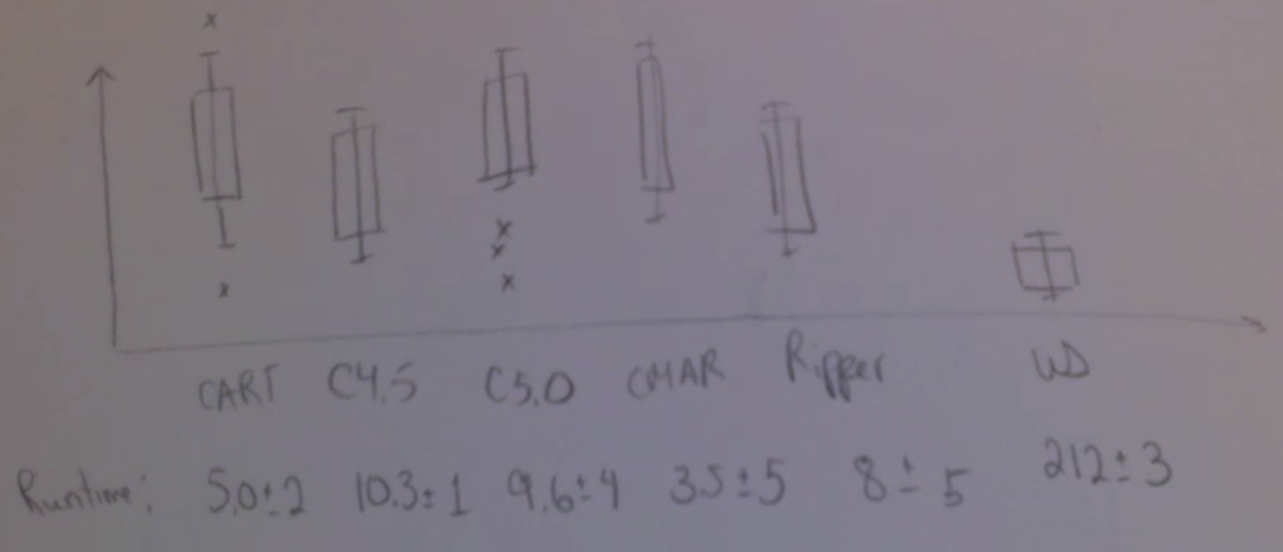
\includegraphics[width=0.75\textwidth]{figs/sketch-comparison.png}
\end{center}
\caption{Comparison with other methods:
Value of the objective for us and a few other algorithms
(CART, C4.5, CBA, CMAR/CPAR, C5.0, Ripper, \dots), and algorithm runtimes,
over ten folds, for one big dataset (box plots)}
\label{fig:comparison}
\end{figure}

\begin{figure}[t!]
\begin{center}
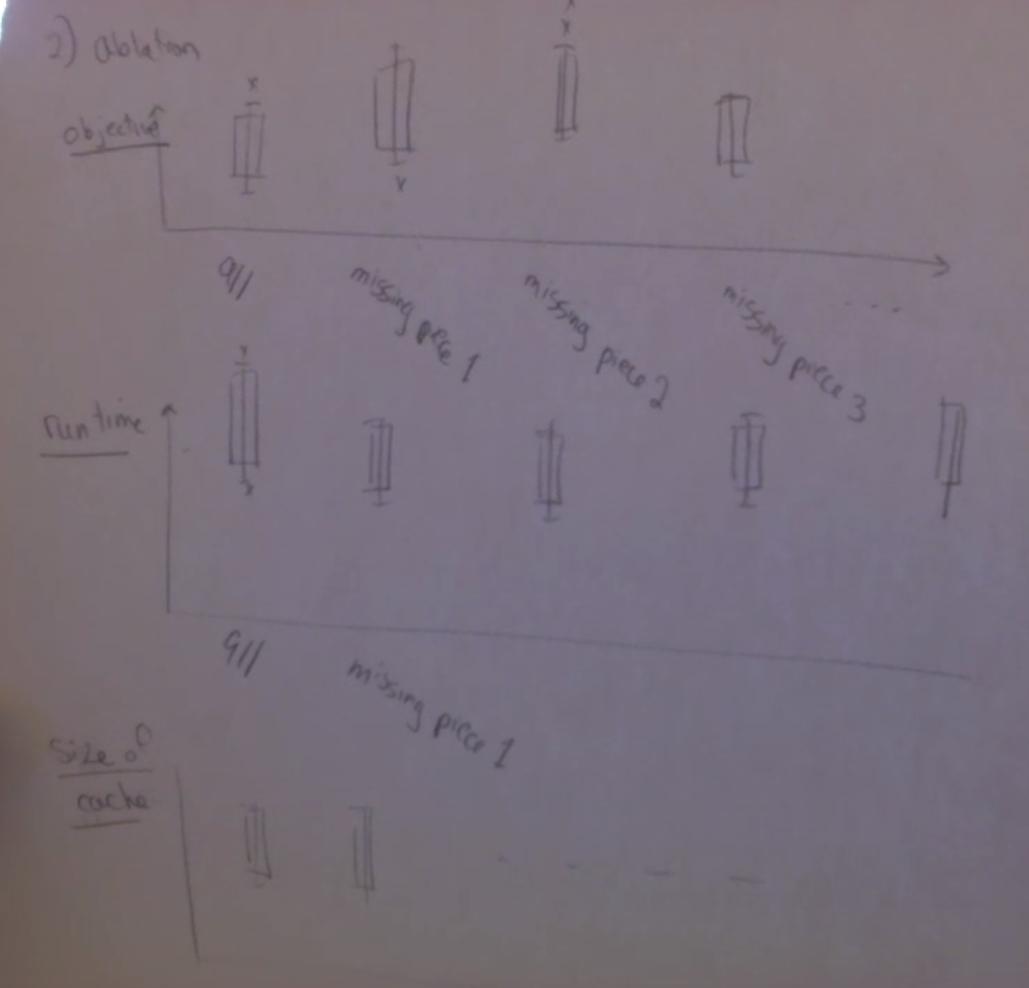
\includegraphics[width=0.75\textwidth]{figs/sketch-ablation.png}
\end{center}
\caption{Ablation experiment:
Show the effect of each ``piece'' at a time,
run X without each in turn and show the difference in either
quality of solution or runtime or amount of memory, size of cache or queue,
where X is a specific implementation
(meaning a specific scheduling policy and node type)}
\label{fig:ablation}
\end{figure}

\begin{figure}[t!]
\begin{center}
\end{center}
\caption{Missing:  Some sort of comparison of different scheduling policies}
\label{fig:scheduling-policy}
\end{figure}

\begin{figure}[t!]
\begin{center}
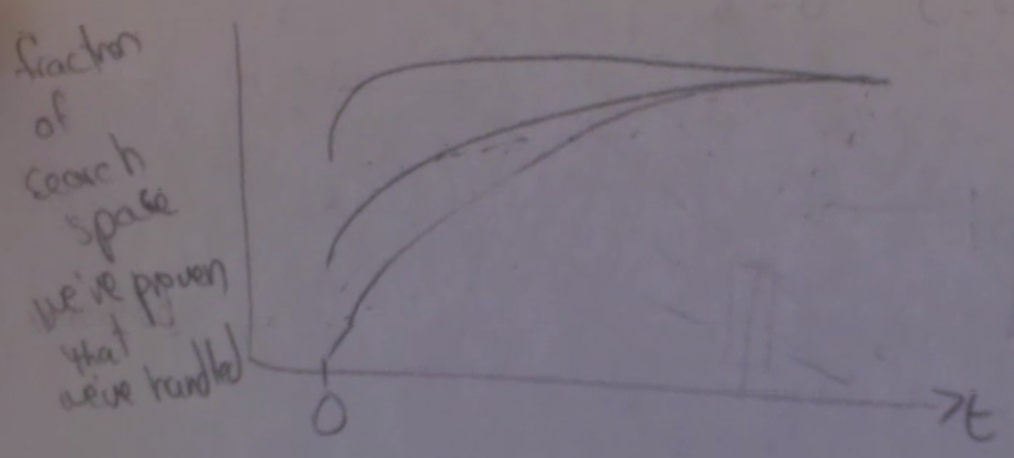
\includegraphics[width=0.65\textwidth]{figs/sketch-search-space.png}
\end{center}
\caption{Fraction of search space we've proven we've handled}
\label{fig:search-space}
\end{figure}

\begin{figure}[t!]
\begin{center}
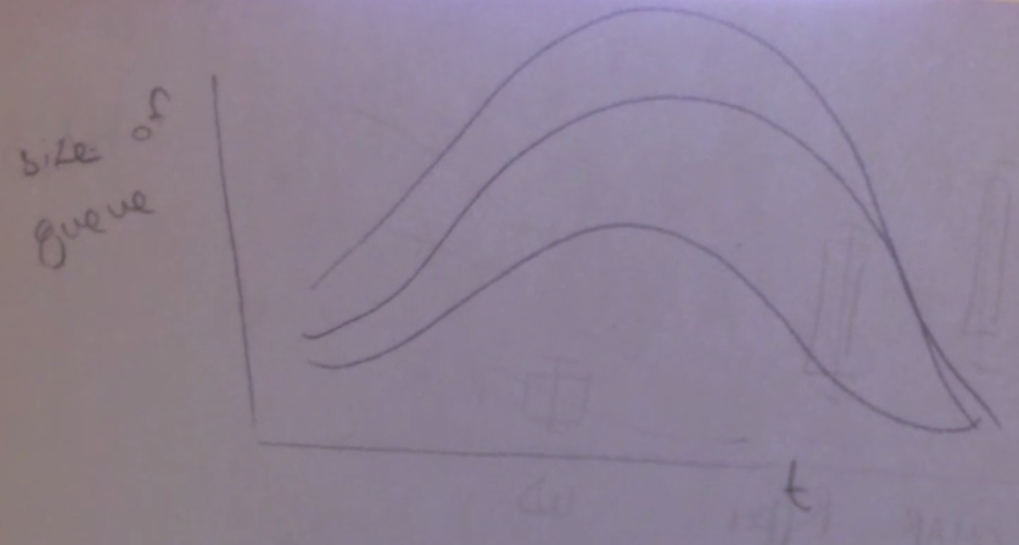
\includegraphics[width=0.65\textwidth]{figs/sketch-queue-size.png}
\end{center}
\caption{Size of queue over time}
\label{fig:queue-size}
\end{figure}

\begin{figure}[t!]
\begin{center}
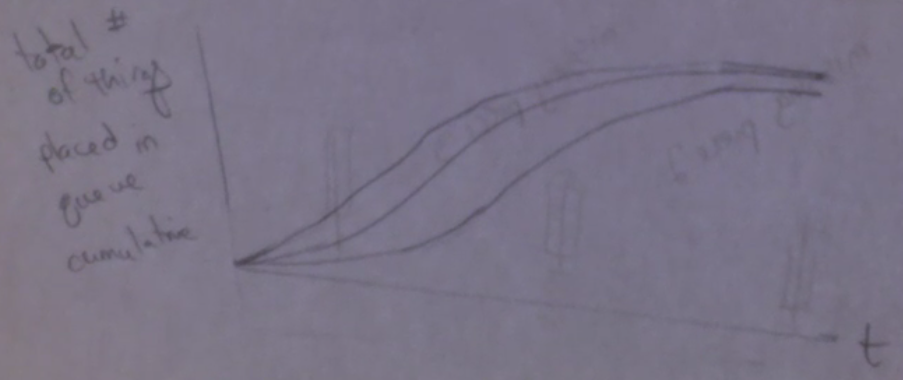
\includegraphics[width=0.65\textwidth]{figs/sketch-queue-cumulative.png}
\end{center}
\caption{Cumulative number of things placed in queue over time}
\label{fig:queue-cumulative}
\end{figure}

\begin{figure}[t!]
\begin{center}
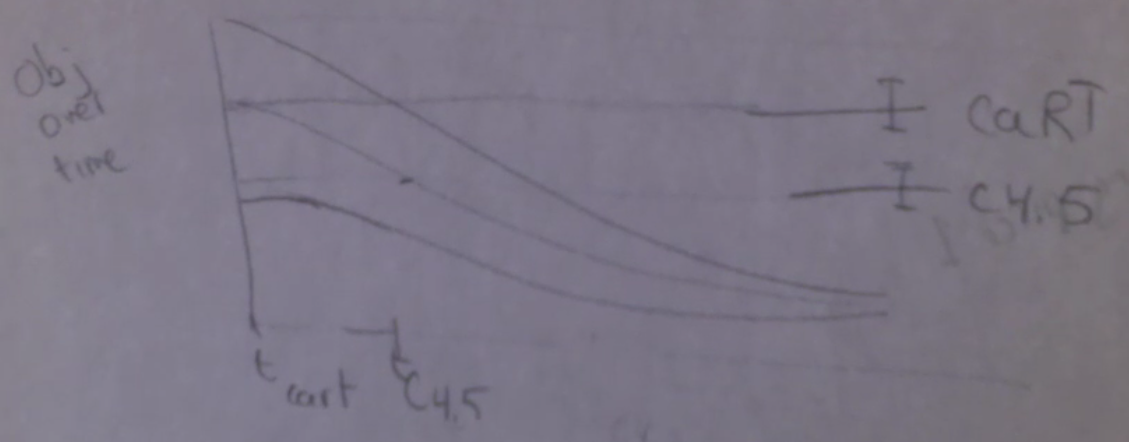
\includegraphics[width=0.65\textwidth]{figs/sketch-objective.png}
\end{center}
\caption{Objective value over time,
with horizontal lines and x-ticks for CART and C4.5}
\label{fig:objective}
\end{figure}

\begin{figure}[t!]
\begin{center}
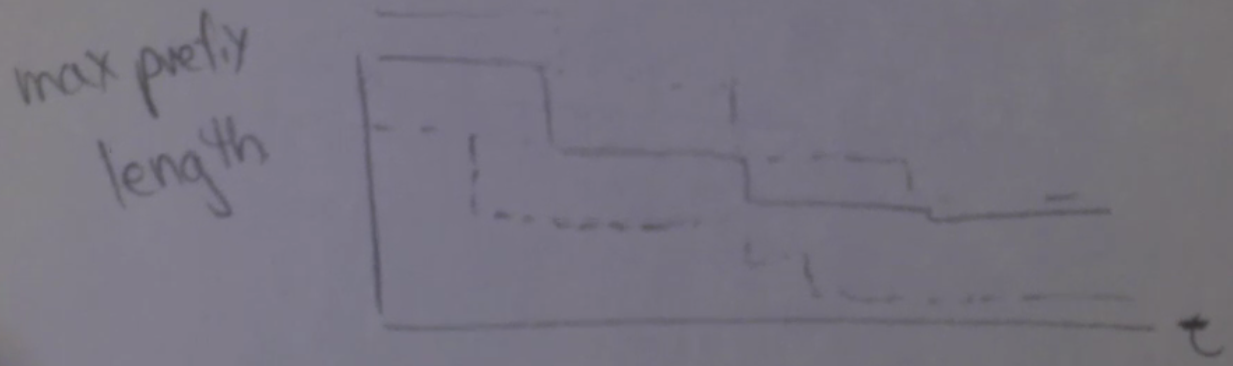
\includegraphics[width=0.65\textwidth]{figs/sketch-max-length.png}
\end{center}
\caption{Max prefix length over time (computed from objective value);
maybe also add the best prefix length over time}
\label{fig:max-length}
\end{figure}
